\documentclass[twoside]{book}

% Packages required by doxygen
\usepackage{fixltx2e}
\usepackage{calc}
\usepackage{doxygen}
\usepackage[export]{adjustbox} % also loads graphicx
\usepackage{graphicx}
\usepackage[utf8]{inputenc}
\usepackage{makeidx}
\usepackage{multicol}
\usepackage{multirow}
\PassOptionsToPackage{warn}{textcomp}
\usepackage{textcomp}
\usepackage[nointegrals]{wasysym}
\usepackage[table]{xcolor}

% Font selection
\usepackage[T1]{fontenc}
\usepackage[scaled=.90]{helvet}
\usepackage{courier}
\usepackage{amssymb}
\usepackage{sectsty}
\renewcommand{\familydefault}{\sfdefault}
\allsectionsfont{%
  \fontseries{bc}\selectfont%
  \color{darkgray}%
}
\renewcommand{\DoxyLabelFont}{%
  \fontseries{bc}\selectfont%
  \color{darkgray}%
}
\newcommand{\+}{\discretionary{\mbox{\scriptsize$\hookleftarrow$}}{}{}}

% Page & text layout
\usepackage{geometry}
\geometry{%
  a4paper,%
  top=2.5cm,%
  bottom=2.5cm,%
  left=2.5cm,%
  right=2.5cm%
}
\tolerance=750
\hfuzz=15pt
\hbadness=750
\setlength{\emergencystretch}{15pt}
\setlength{\parindent}{0cm}
\setlength{\parskip}{3ex plus 2ex minus 2ex}
\makeatletter
\renewcommand{\paragraph}{%
  \@startsection{paragraph}{4}{0ex}{-1.0ex}{1.0ex}{%
    \normalfont\normalsize\bfseries\SS@parafont%
  }%
}
\renewcommand{\subparagraph}{%
  \@startsection{subparagraph}{5}{0ex}{-1.0ex}{1.0ex}{%
    \normalfont\normalsize\bfseries\SS@subparafont%
  }%
}
\makeatother

% Headers & footers
\usepackage{fancyhdr}
\pagestyle{fancyplain}
\fancyhead[LE]{\fancyplain{}{\bfseries\thepage}}
\fancyhead[CE]{\fancyplain{}{}}
\fancyhead[RE]{\fancyplain{}{\bfseries\leftmark}}
\fancyhead[LO]{\fancyplain{}{\bfseries\rightmark}}
\fancyhead[CO]{\fancyplain{}{}}
\fancyhead[RO]{\fancyplain{}{\bfseries\thepage}}
\fancyfoot[LE]{\fancyplain{}{}}
\fancyfoot[CE]{\fancyplain{}{}}
\fancyfoot[RE]{\fancyplain{}{\bfseries\scriptsize Generated by Doxygen }}
\fancyfoot[LO]{\fancyplain{}{\bfseries\scriptsize Generated by Doxygen }}
\fancyfoot[CO]{\fancyplain{}{}}
\fancyfoot[RO]{\fancyplain{}{}}
\renewcommand{\footrulewidth}{0.4pt}
\renewcommand{\chaptermark}[1]{%
  \markboth{#1}{}%
}
\renewcommand{\sectionmark}[1]{%
  \markright{\thesection\ #1}%
}

% Indices & bibliography
\usepackage{natbib}
\usepackage[titles]{tocloft}
\setcounter{tocdepth}{3}
\setcounter{secnumdepth}{5}
\makeindex

% Hyperlinks (required, but should be loaded last)
\usepackage{ifpdf}
\ifpdf
  \usepackage[pdftex,pagebackref=true]{hyperref}
\else
  \usepackage[ps2pdf,pagebackref=true]{hyperref}
\fi
\hypersetup{%
  colorlinks=true,%
  linkcolor=blue,%
  citecolor=blue,%
  unicode%
}

% Custom commands
\newcommand{\clearemptydoublepage}{%
  \newpage{\pagestyle{empty}\cleardoublepage}%
}

\usepackage{caption}
\captionsetup{labelsep=space,justification=centering,font={bf},singlelinecheck=off,skip=4pt,position=top}

%===== C O N T E N T S =====

\begin{document}

% Titlepage & ToC
\hypersetup{pageanchor=false,
             bookmarksnumbered=true,
             pdfencoding=unicode
            }
\pagenumbering{roman}
\begin{titlepage}
\vspace*{7cm}
\begin{center}%
{\Large Exp\+\_\+\+Lab\+\_\+\+Assignments }\\
\vspace*{1cm}
{\large Generated by Doxygen 1.8.11}\\
\end{center}
\end{titlepage}
\clearemptydoublepage
\tableofcontents
\clearemptydoublepage
\pagenumbering{arabic}
\hypersetup{pageanchor=true}

%--- Begin generated contents ---
\chapter{Hierarchical Index}
\section{Class Hierarchy}
This inheritance list is sorted roughly, but not completely, alphabetically\+:\begin{DoxyCompactList}
\item \contentsline{section}{state\+\_\+manager.\+coordinates\+\_\+from\+\_\+picture}{\pageref{classstate__manager_1_1coordinates__from__picture}}{}
\item State\begin{DoxyCompactList}
\item \contentsline{section}{state\+\_\+manager.\+M\+I\+R\+O\+\_\+\+Normal}{\pageref{classstate__manager_1_1MIRO__Normal}}{}
\item \contentsline{section}{state\+\_\+manager.\+M\+I\+R\+O\+\_\+\+Play}{\pageref{classstate__manager_1_1MIRO__Play}}{}
\item \contentsline{section}{state\+\_\+manager.\+M\+I\+R\+O\+\_\+\+Sleep}{\pageref{classstate__manager_1_1MIRO__Sleep}}{}
\end{DoxyCompactList}
\end{DoxyCompactList}

\chapter{Class Index}
\section{Class List}
Here are the classes, structs, unions and interfaces with brief descriptions\+:\begin{DoxyCompactList}
\item\contentsline{section}{\hyperlink{classstate__manager_1_1coordinates__from__picture}{state\+\_\+manager.\+coordinates\+\_\+from\+\_\+picture} }{\pageref{classstate__manager_1_1coordinates__from__picture}}{}
\item\contentsline{section}{\hyperlink{classstate__manager_1_1MIRO__Normal}{state\+\_\+manager.\+M\+I\+R\+O\+\_\+\+Normal} }{\pageref{classstate__manager_1_1MIRO__Normal}}{}
\item\contentsline{section}{\hyperlink{classstate__manager_1_1MIRO__Play}{state\+\_\+manager.\+M\+I\+R\+O\+\_\+\+Play} }{\pageref{classstate__manager_1_1MIRO__Play}}{}
\item\contentsline{section}{\hyperlink{classstate__manager_1_1MIRO__Sleep}{state\+\_\+manager.\+M\+I\+R\+O\+\_\+\+Sleep} }{\pageref{classstate__manager_1_1MIRO__Sleep}}{}
\end{DoxyCompactList}

\chapter{File Index}
\section{File List}
Here is a list of all documented files with brief descriptions\+:\begin{DoxyCompactList}
\item\contentsline{section}{src/\hyperlink{geometry__grounding_8py}{geometry\+\_\+grounding.\+py} \\*This node transforms a command into two x,y coordinates }{\pageref{geometry__grounding_8py}}{}
\item\contentsline{section}{src/\hyperlink{printInfo_8py}{print\+Info.\+py} \\*This node prints informations about target position, reached position, state }{\pageref{printInfo_8py}}{}
\item\contentsline{section}{src/\hyperlink{robot__motion__controller_8py}{robot\+\_\+motion\+\_\+controller.\+py} \\*This node allows to move the robot from the current to the target position }{\pageref{robot__motion__controller_8py}}{}
\item\contentsline{section}{src/{\bfseries state\+\_\+manager.\+py} }{\pageref{state__manager_8py}}{}
\end{DoxyCompactList}

\chapter{Class Documentation}
\hypertarget{classstate__manager_1_1coordinates__from__picture}{}\section{state\+\_\+manager.\+coordinates\+\_\+from\+\_\+picture Class Reference}
\label{classstate__manager_1_1coordinates__from__picture}\index{state\+\_\+manager.\+coordinates\+\_\+from\+\_\+picture@{state\+\_\+manager.\+coordinates\+\_\+from\+\_\+picture}}
\subsection*{Public Member Functions}
\begin{DoxyCompactItemize}
\item 
def \hyperlink{classstate__manager_1_1coordinates__from__picture_a1cfcda6b1096fe141974378b701b9402}{\+\_\+\+\_\+init\+\_\+\+\_\+} (self, name)
\item 
def \hyperlink{classstate__manager_1_1coordinates__from__picture_a480690c0f23cc43b67c9ed8343c41e19}{add\+\_\+data} (self, img\+\_\+person\+\_\+posx, img\+\_\+person\+\_\+posy, img\+\_\+gesture\+\_\+posx, img\+\_\+gesture\+\_\+posy)
\end{DoxyCompactItemize}
\subsection*{Public Attributes}
\begin{DoxyCompactItemize}
\item 
{\bfseries person\+\_\+posx}\hypertarget{classstate__manager_1_1coordinates__from__picture_a9c453774ff4cc0644deb040473934bdc}{}\label{classstate__manager_1_1coordinates__from__picture_a9c453774ff4cc0644deb040473934bdc}

\item 
{\bfseries person\+\_\+posy}\hypertarget{classstate__manager_1_1coordinates__from__picture_aabe7e4fb692c99db14d42b6bdd79a656}{}\label{classstate__manager_1_1coordinates__from__picture_aabe7e4fb692c99db14d42b6bdd79a656}

\item 
{\bfseries gesture\+\_\+posx}\hypertarget{classstate__manager_1_1coordinates__from__picture_a945328edc4ceccd3ab9e72b44e785a37}{}\label{classstate__manager_1_1coordinates__from__picture_a945328edc4ceccd3ab9e72b44e785a37}

\item 
{\bfseries gesture\+\_\+posy}\hypertarget{classstate__manager_1_1coordinates__from__picture_a4e1df084f290ebf50ce72a6eff5f938d}{}\label{classstate__manager_1_1coordinates__from__picture_a4e1df084f290ebf50ce72a6eff5f938d}

\end{DoxyCompactItemize}


\subsection{Detailed Description}
\begin{DoxyVerb}Simulates a camera frame and the information it contains.
\end{DoxyVerb}
 

\subsection{Constructor \& Destructor Documentation}
\index{state\+\_\+manager\+::coordinates\+\_\+from\+\_\+picture@{state\+\_\+manager\+::coordinates\+\_\+from\+\_\+picture}!\+\_\+\+\_\+init\+\_\+\+\_\+@{\+\_\+\+\_\+init\+\_\+\+\_\+}}
\index{\+\_\+\+\_\+init\+\_\+\+\_\+@{\+\_\+\+\_\+init\+\_\+\+\_\+}!state\+\_\+manager\+::coordinates\+\_\+from\+\_\+picture@{state\+\_\+manager\+::coordinates\+\_\+from\+\_\+picture}}
\subsubsection[{\texorpdfstring{\+\_\+\+\_\+init\+\_\+\+\_\+(self, name)}{__init__(self, name)}}]{\setlength{\rightskip}{0pt plus 5cm}def state\+\_\+manager.\+coordinates\+\_\+from\+\_\+picture.\+\_\+\+\_\+init\+\_\+\+\_\+ (
\begin{DoxyParamCaption}
\item[{}]{self, }
\item[{}]{name}
\end{DoxyParamCaption}
)}\hypertarget{classstate__manager_1_1coordinates__from__picture_a1cfcda6b1096fe141974378b701b9402}{}\label{classstate__manager_1_1coordinates__from__picture_a1cfcda6b1096fe141974378b701b9402}
\begin{DoxyVerb}Init function for coordinates_from_picture class.
\end{DoxyVerb}
 

\subsection{Member Function Documentation}
\index{state\+\_\+manager\+::coordinates\+\_\+from\+\_\+picture@{state\+\_\+manager\+::coordinates\+\_\+from\+\_\+picture}!add\+\_\+data@{add\+\_\+data}}
\index{add\+\_\+data@{add\+\_\+data}!state\+\_\+manager\+::coordinates\+\_\+from\+\_\+picture@{state\+\_\+manager\+::coordinates\+\_\+from\+\_\+picture}}
\subsubsection[{\texorpdfstring{add\+\_\+data(self, img\+\_\+person\+\_\+posx, img\+\_\+person\+\_\+posy, img\+\_\+gesture\+\_\+posx, img\+\_\+gesture\+\_\+posy)}{add_data(self, img_person_posx, img_person_posy, img_gesture_posx, img_gesture_posy)}}]{\setlength{\rightskip}{0pt plus 5cm}def state\+\_\+manager.\+coordinates\+\_\+from\+\_\+picture.\+add\+\_\+data (
\begin{DoxyParamCaption}
\item[{}]{self, }
\item[{}]{img\+\_\+person\+\_\+posx, }
\item[{}]{img\+\_\+person\+\_\+posy, }
\item[{}]{img\+\_\+gesture\+\_\+posx, }
\item[{}]{img\+\_\+gesture\+\_\+posy}
\end{DoxyParamCaption}
)}\hypertarget{classstate__manager_1_1coordinates__from__picture_a480690c0f23cc43b67c9ed8343c41e19}{}\label{classstate__manager_1_1coordinates__from__picture_a480690c0f23cc43b67c9ed8343c41e19}
\begin{DoxyVerb}Add data function for coordinates_from_picture class.
\end{DoxyVerb}
 

The documentation for this class was generated from the following file\+:\begin{DoxyCompactItemize}
\item 
/home/chiara/catkin\+\_\+ws/src/\+Exp\+\_\+lab\+\_\+assignments/src/state\+\_\+manager.\+py\end{DoxyCompactItemize}

\hypertarget{classstate__manager_1_1MIRO__Normal}{}\section{state\+\_\+manager.\+M\+I\+R\+O\+\_\+\+Normal Class Reference}
\label{classstate__manager_1_1MIRO__Normal}\index{state\+\_\+manager.\+M\+I\+R\+O\+\_\+\+Normal@{state\+\_\+manager.\+M\+I\+R\+O\+\_\+\+Normal}}


Normal state of the smach machine.  




Inheritance diagram for state\+\_\+manager.\+M\+I\+R\+O\+\_\+\+Normal\+:
\nopagebreak
\begin{figure}[H]
\begin{center}
\leavevmode
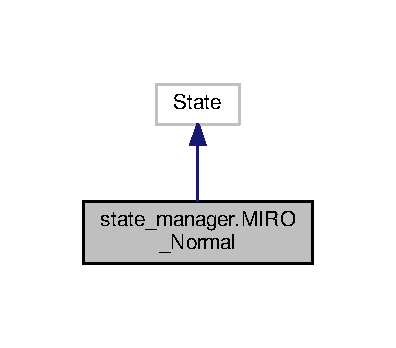
\includegraphics[width=190pt]{classstate__manager_1_1MIRO__Normal__inherit__graph}
\end{center}
\end{figure}


Collaboration diagram for state\+\_\+manager.\+M\+I\+R\+O\+\_\+\+Normal\+:
\nopagebreak
\begin{figure}[H]
\begin{center}
\leavevmode
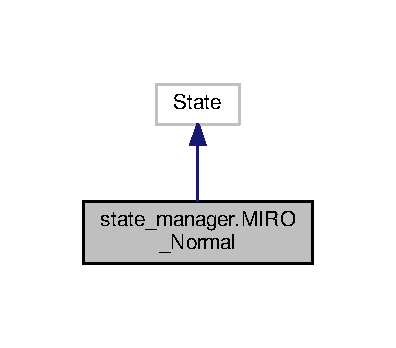
\includegraphics[width=190pt]{classstate__manager_1_1MIRO__Normal__coll__graph}
\end{center}
\end{figure}
\subsection*{Public Member Functions}
\begin{DoxyCompactItemize}
\item 
def \hyperlink{classstate__manager_1_1MIRO__Normal_a36a3ee79119b52beeebd6ee8c04d9501}{\+\_\+\+\_\+init\+\_\+\+\_\+} (self)
\begin{DoxyCompactList}\small\item\em Init function for smach machine normal state. \end{DoxyCompactList}\item 
def \hyperlink{classstate__manager_1_1MIRO__Normal_a4133da39ee6ec170623fc1d457b0729a}{execute} (self, userdata)
\begin{DoxyCompactList}\small\item\em Smach machine state normal actions\+: Listens to user\+: if user says \char`\"{}\+Play\char`\"{} or \char`\"{}\+Hey buddy\char`\"{} it outputs command to enter play state. \end{DoxyCompactList}\end{DoxyCompactItemize}


\subsection{Detailed Description}
Normal state of the smach machine. 



Definition at line 106 of file state\+\_\+manager.\+py.



\subsection{Constructor \& Destructor Documentation}
\index{state\+\_\+manager\+::\+M\+I\+R\+O\+\_\+\+Normal@{state\+\_\+manager\+::\+M\+I\+R\+O\+\_\+\+Normal}!\+\_\+\+\_\+init\+\_\+\+\_\+@{\+\_\+\+\_\+init\+\_\+\+\_\+}}
\index{\+\_\+\+\_\+init\+\_\+\+\_\+@{\+\_\+\+\_\+init\+\_\+\+\_\+}!state\+\_\+manager\+::\+M\+I\+R\+O\+\_\+\+Normal@{state\+\_\+manager\+::\+M\+I\+R\+O\+\_\+\+Normal}}
\subsubsection[{\texorpdfstring{\+\_\+\+\_\+init\+\_\+\+\_\+(self)}{__init__(self)}}]{\setlength{\rightskip}{0pt plus 5cm}def state\+\_\+manager.\+M\+I\+R\+O\+\_\+\+Normal.\+\_\+\+\_\+init\+\_\+\+\_\+ (
\begin{DoxyParamCaption}
\item[{}]{self}
\end{DoxyParamCaption}
)}\hypertarget{classstate__manager_1_1MIRO__Normal_a36a3ee79119b52beeebd6ee8c04d9501}{}\label{classstate__manager_1_1MIRO__Normal_a36a3ee79119b52beeebd6ee8c04d9501}


Init function for smach machine normal state. 



Definition at line 109 of file state\+\_\+manager.\+py.


\begin{DoxyCode}
109     \textcolor{keyword}{def }\hyperlink{classstate__manager_1_1MIRO__Normal_a36a3ee79119b52beeebd6ee8c04d9501}{\_\_init\_\_}(self):
110 
111         smach.State.\_\_init\_\_(self,
112                              outcomes=[\textcolor{stringliteral}{'sleep\_command'}, \textcolor{stringliteral}{'play\_command'}])
113 
\end{DoxyCode}


\subsection{Member Function Documentation}
\index{state\+\_\+manager\+::\+M\+I\+R\+O\+\_\+\+Normal@{state\+\_\+manager\+::\+M\+I\+R\+O\+\_\+\+Normal}!execute@{execute}}
\index{execute@{execute}!state\+\_\+manager\+::\+M\+I\+R\+O\+\_\+\+Normal@{state\+\_\+manager\+::\+M\+I\+R\+O\+\_\+\+Normal}}
\subsubsection[{\texorpdfstring{execute(self, userdata)}{execute(self, userdata)}}]{\setlength{\rightskip}{0pt plus 5cm}def state\+\_\+manager.\+M\+I\+R\+O\+\_\+\+Normal.\+execute (
\begin{DoxyParamCaption}
\item[{}]{self, }
\item[{}]{userdata}
\end{DoxyParamCaption}
)}\hypertarget{classstate__manager_1_1MIRO__Normal_a4133da39ee6ec170623fc1d457b0729a}{}\label{classstate__manager_1_1MIRO__Normal_a4133da39ee6ec170623fc1d457b0729a}


Smach machine state normal actions\+: Listens to user\+: if user says \char`\"{}\+Play\char`\"{} or \char`\"{}\+Hey buddy\char`\"{} it outputs command to enter play state. 

If user says nothing, it goes to random positions for a while (n loops) then outputs command to enter sleep state. \begin{DoxyReturn}{Returns}
c\+: command to switch between states. 
\end{DoxyReturn}


Definition at line 118 of file state\+\_\+manager.\+py.


\begin{DoxyCode}
118     \textcolor{keyword}{def }\hyperlink{classstate__manager_1_1MIRO__Normal_a4133da39ee6ec170623fc1d457b0729a}{execute}(self, userdata):
119 
120         \textcolor{comment}{# Set state parameter}
121         rospy.set\_param(\textcolor{stringliteral}{'state'}, \textcolor{stringliteral}{'NORMAL'})
122 
123         \textcolor{keywordflow}{for} i \textcolor{keywordflow}{in} range(0, LOOPS):
124 
125             \textcolor{comment}{# Checks if user is speaking}
126             user\_command = user\_says(0)
127 
128             \textcolor{comment}{# If user is calling MIRO, enter play state}
129             \textcolor{keywordflow}{if} user\_command == \textcolor{stringliteral}{'hey buddy'} \textcolor{keywordflow}{or} user\_command == \textcolor{stringliteral}{'play'}:
130                 c = \textcolor{stringliteral}{'play\_command'}
131                 \textcolor{keywordflow}{return} c
132 
133             \textcolor{comment}{# Else wander around}
134             \textcolor{keywordflow}{else}:
135                 \textcolor{comment}{# Wait to be ready}
136                 \textcolor{keywordflow}{while} rospy.get\_param(\textcolor{stringliteral}{'arrived'}) == 0:
137                     time.sleep(1)
138                 rospy.set\_param(\textcolor{stringliteral}{'arrived'}, 0)
139 
140                 normal\_command = \textcolor{stringliteral}{'go\_rand'}
141 
142                 \textcolor{comment}{# Publish normal command}
143                 pub.publish(normal\_command)
144                 time.sleep(3)
145 
146             \textcolor{comment}{# Randomly decide to sleep, enter sleep state}
147             \textcolor{keywordflow}{if} random.randrange(0, 5) == 1:
148                 c = \textcolor{stringliteral}{'sleep\_command'}
149                 \textcolor{keywordflow}{return} c
150 
151         \textcolor{keywordflow}{return} \textcolor{stringliteral}{'sleep\_command'}
152 
\end{DoxyCode}


The documentation for this class was generated from the following file\+:\begin{DoxyCompactItemize}
\item 
src/state\+\_\+manager.\+py\end{DoxyCompactItemize}

\hypertarget{classstate__manager_1_1MIRO__Play}{}\section{state\+\_\+manager.\+M\+I\+R\+O\+\_\+\+Play Class Reference}
\label{classstate__manager_1_1MIRO__Play}\index{state\+\_\+manager.\+M\+I\+R\+O\+\_\+\+Play@{state\+\_\+manager.\+M\+I\+R\+O\+\_\+\+Play}}


Play state of the smach machine.  




Inheritance diagram for state\+\_\+manager.\+M\+I\+R\+O\+\_\+\+Play\+:
\nopagebreak
\begin{figure}[H]
\begin{center}
\leavevmode
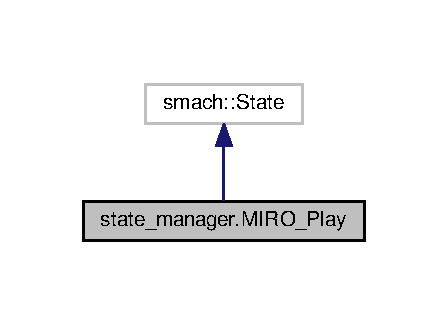
\includegraphics[width=215pt]{classstate__manager_1_1MIRO__Play__inherit__graph}
\end{center}
\end{figure}


Collaboration diagram for state\+\_\+manager.\+M\+I\+R\+O\+\_\+\+Play\+:
\nopagebreak
\begin{figure}[H]
\begin{center}
\leavevmode
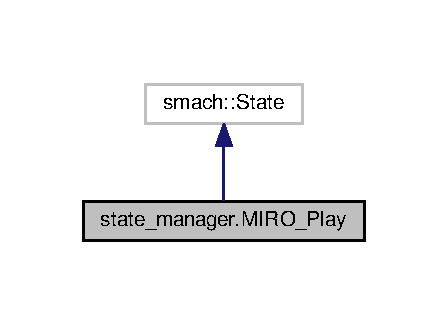
\includegraphics[width=215pt]{classstate__manager_1_1MIRO__Play__coll__graph}
\end{center}
\end{figure}
\subsection*{Public Member Functions}
\begin{DoxyCompactItemize}
\item 
def \hyperlink{classstate__manager_1_1MIRO__Play_a863ae1958460cf6bf33faaba597fc5a2}{\+\_\+\+\_\+init\+\_\+\+\_\+} (self)
\begin{DoxyCompactList}\small\item\em Init function for smach machine play state. \end{DoxyCompactList}\item 
def \hyperlink{classstate__manager_1_1MIRO__Play_a781db4be4fcbb313c46097a8fdf06275}{execute} (self, userdata)
\begin{DoxyCompactList}\small\item\em Smach machine state play actions\+: Looks at user, saves his coordinates as next position, publishes them (goes toward the human). \end{DoxyCompactList}\end{DoxyCompactItemize}


\subsection{Detailed Description}
Play state of the smach machine. 



Definition at line 154 of file state\+\_\+manager.\+py.



\subsection{Constructor \& Destructor Documentation}
\index{state\+\_\+manager\+::\+M\+I\+R\+O\+\_\+\+Play@{state\+\_\+manager\+::\+M\+I\+R\+O\+\_\+\+Play}!\+\_\+\+\_\+init\+\_\+\+\_\+@{\+\_\+\+\_\+init\+\_\+\+\_\+}}
\index{\+\_\+\+\_\+init\+\_\+\+\_\+@{\+\_\+\+\_\+init\+\_\+\+\_\+}!state\+\_\+manager\+::\+M\+I\+R\+O\+\_\+\+Play@{state\+\_\+manager\+::\+M\+I\+R\+O\+\_\+\+Play}}
\subsubsection[{\texorpdfstring{\+\_\+\+\_\+init\+\_\+\+\_\+(self)}{__init__(self)}}]{\setlength{\rightskip}{0pt plus 5cm}def state\+\_\+manager.\+M\+I\+R\+O\+\_\+\+Play.\+\_\+\+\_\+init\+\_\+\+\_\+ (
\begin{DoxyParamCaption}
\item[{}]{self}
\end{DoxyParamCaption}
)}\hypertarget{classstate__manager_1_1MIRO__Play_a863ae1958460cf6bf33faaba597fc5a2}{}\label{classstate__manager_1_1MIRO__Play_a863ae1958460cf6bf33faaba597fc5a2}


Init function for smach machine play state. 



Definition at line 157 of file state\+\_\+manager.\+py.


\begin{DoxyCode}
157     \textcolor{keyword}{def }\hyperlink{classstate__manager_1_1MIRO__Play_a863ae1958460cf6bf33faaba597fc5a2}{\_\_init\_\_}(self):
158 
159         smach.State.\_\_init\_\_(self,
160                              outcomes=[\textcolor{stringliteral}{'normal\_command'}])
161 
\end{DoxyCode}


\subsection{Member Function Documentation}
\index{state\+\_\+manager\+::\+M\+I\+R\+O\+\_\+\+Play@{state\+\_\+manager\+::\+M\+I\+R\+O\+\_\+\+Play}!execute@{execute}}
\index{execute@{execute}!state\+\_\+manager\+::\+M\+I\+R\+O\+\_\+\+Play@{state\+\_\+manager\+::\+M\+I\+R\+O\+\_\+\+Play}}
\subsubsection[{\texorpdfstring{execute(self, userdata)}{execute(self, userdata)}}]{\setlength{\rightskip}{0pt plus 5cm}def state\+\_\+manager.\+M\+I\+R\+O\+\_\+\+Play.\+execute (
\begin{DoxyParamCaption}
\item[{}]{self, }
\item[{}]{userdata}
\end{DoxyParamCaption}
)}\hypertarget{classstate__manager_1_1MIRO__Play_a781db4be4fcbb313c46097a8fdf06275}{}\label{classstate__manager_1_1MIRO__Play_a781db4be4fcbb313c46097a8fdf06275}


Smach machine state play actions\+: Looks at user, saves his coordinates as next position, publishes them (goes toward the human). 

It then listens to the user. If user says \char`\"{}go to posx posy\char`\"{}, publishes the coordinates (goes to the point). If user says \char`\"{}\+Hey buddy\char`\"{} or \char`\"{}\+Play\char`\"{} it waits. If user says nothing, it looks for the user gesture to go somewhere, and publishes the coordinate he receives (goes to the point). This repeates for a while (n loops) then the robot enters normal state again. \begin{DoxyReturn}{Returns}
c\+: command to switch between states. 
\end{DoxyReturn}


Definition at line 169 of file state\+\_\+manager.\+py.


\begin{DoxyCode}
169     \textcolor{keyword}{def }\hyperlink{classstate__manager_1_1MIRO__Play_a781db4be4fcbb313c46097a8fdf06275}{execute}(self, userdata):
170 
171         \textcolor{comment}{# Set state parameter}
172         rospy.set\_param(\textcolor{stringliteral}{'state'}, \textcolor{stringliteral}{'PLAY STATE'})
173 
174         \textcolor{keywordflow}{for} i \textcolor{keywordflow}{in} range(0, LOOPS):
175 
176             \textcolor{comment}{# Check where user is (assumption:he is there, since he called MIRO)}
177             user\_camera = user\_does()
178             \textcolor{comment}{# Save user position}
179             user\_position = \textcolor{stringliteral}{"go to %d %d"} % (
180                 user\_camera[0], user\_camera[1])
181 
182             \textcolor{comment}{# Wait to be ready}
183             \textcolor{keywordflow}{while} rospy.get\_param(\textcolor{stringliteral}{'arrived'}) == 0:
184                 time.sleep(1)
185             rospy.set\_param(\textcolor{stringliteral}{'arrived'}, 0)
186 
187             \textcolor{comment}{# Go to user}
188             pub.publish(user\_position)
189             time.sleep(3)
190 
191             \textcolor{comment}{# Listen to user}
192             user\_command = user\_says(1)
193 
194             \textcolor{comment}{# If user says to go somewhere...}
195             \textcolor{keywordflow}{if} \textcolor{stringliteral}{'go'} \textcolor{keywordflow}{in} user\_command \textcolor{keywordflow}{and} \textcolor{stringliteral}{'to'} \textcolor{keywordflow}{in} user\_command:
196                 check\_int = [int(s)
197                              \textcolor{keywordflow}{for} s \textcolor{keywordflow}{in} user\_command.split() \textcolor{keywordflow}{if} s.isdigit()]
198                 \textcolor{comment}{# ... and he actually gives you two coordinates...}
199 
200                 \textcolor{keywordflow}{if} len(check\_int) != 2:
201                     rospy.logerr(\textcolor{stringliteral}{'Wrong command'})
202                     \textcolor{keywordflow}{break}
203 
204                 \textcolor{comment}{# Wait to be ready}
205                 \textcolor{keywordflow}{while} rospy.get\_param(\textcolor{stringliteral}{'arrived'}) == 0:
206                     time.sleep(1)
207                 rospy.set\_param(\textcolor{stringliteral}{'arrived'}, 0)
208 
209                 \textcolor{comment}{# ...Go to position}
210                 pub.publish(user\_command)
211                 time.sleep(3)
212 
213             \textcolor{comment}{# If user says he wants to play: wait}
214             \textcolor{keywordflow}{elif} user\_command == \textcolor{stringliteral}{'hey buddy'} \textcolor{keywordflow}{or} user\_command == \textcolor{stringliteral}{'play'}:
215                 time.sleep(2)
216 
217             \textcolor{comment}{# If user sayes nothing}
218             \textcolor{keywordflow}{else}:
219                 \textcolor{comment}{# Look at user gesture}
220                 user\_gesture = user\_does()
221                 user\_command = \textcolor{stringliteral}{"go to %d %d"} % (
222                     user\_camera.gesture\_posx, user\_camera.gesture\_posy)
223 
224                 \textcolor{keywordflow}{while} rospy.get\_param(\textcolor{stringliteral}{'arrived'}) == 0:
225                     time.sleep(1)
226                 rospy.set\_param(\textcolor{stringliteral}{'arrived'}, 0)
227 
228                 \textcolor{comment}{# Go to position}
229                 pub.publish(user\_command)
230                 time.sleep(3)
231 
232         c = \textcolor{stringliteral}{'normal\_command'}
233         \textcolor{keywordflow}{return} c
234 
\end{DoxyCode}


The documentation for this class was generated from the following file\+:\begin{DoxyCompactItemize}
\item 
src/state\+\_\+manager.\+py\end{DoxyCompactItemize}

\hypertarget{classstate__manager_1_1MIRO__Sleep}{}\section{state\+\_\+manager.\+M\+I\+R\+O\+\_\+\+Sleep Class Reference}
\label{classstate__manager_1_1MIRO__Sleep}\index{state\+\_\+manager.\+M\+I\+R\+O\+\_\+\+Sleep@{state\+\_\+manager.\+M\+I\+R\+O\+\_\+\+Sleep}}


Sleep state of the smach machine.  




Inheritance diagram for state\+\_\+manager.\+M\+I\+R\+O\+\_\+\+Sleep\+:
\nopagebreak
\begin{figure}[H]
\begin{center}
\leavevmode
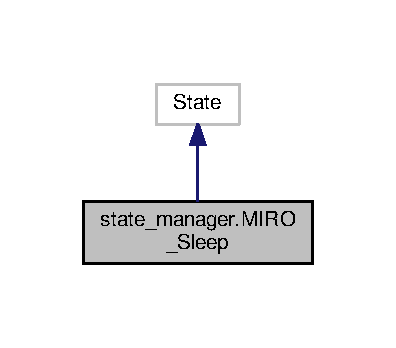
\includegraphics[width=190pt]{classstate__manager_1_1MIRO__Sleep__inherit__graph}
\end{center}
\end{figure}


Collaboration diagram for state\+\_\+manager.\+M\+I\+R\+O\+\_\+\+Sleep\+:
\nopagebreak
\begin{figure}[H]
\begin{center}
\leavevmode
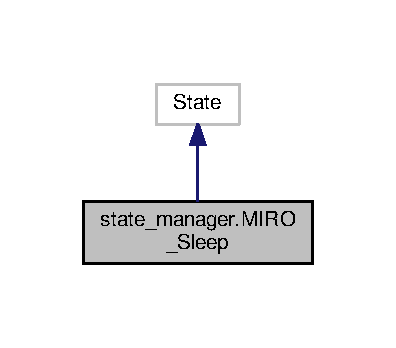
\includegraphics[width=190pt]{classstate__manager_1_1MIRO__Sleep__coll__graph}
\end{center}
\end{figure}
\subsection*{Public Member Functions}
\begin{DoxyCompactItemize}
\item 
def \hyperlink{classstate__manager_1_1MIRO__Sleep_a1e0695b96023b2c827bd28d9b0c11bfb}{\+\_\+\+\_\+init\+\_\+\+\_\+} (self)
\begin{DoxyCompactList}\small\item\em Init function for smach machine sleep state. \end{DoxyCompactList}\item 
def \hyperlink{classstate__manager_1_1MIRO__Sleep_acda704c667aad40c16f10d7c705b1b2e}{execute} (self, userdata)
\begin{DoxyCompactList}\small\item\em Smach machine state sleep actions\+: Publishes \char`\"{}go home\char`\"{} command, waits (\char`\"{}sleeps\char`\"{}) and outputs command to enter normal state. \end{DoxyCompactList}\end{DoxyCompactItemize}


\subsection{Detailed Description}
Sleep state of the smach machine. 



Definition at line 73 of file state\+\_\+manager.\+py.



\subsection{Constructor \& Destructor Documentation}
\index{state\+\_\+manager\+::\+M\+I\+R\+O\+\_\+\+Sleep@{state\+\_\+manager\+::\+M\+I\+R\+O\+\_\+\+Sleep}!\+\_\+\+\_\+init\+\_\+\+\_\+@{\+\_\+\+\_\+init\+\_\+\+\_\+}}
\index{\+\_\+\+\_\+init\+\_\+\+\_\+@{\+\_\+\+\_\+init\+\_\+\+\_\+}!state\+\_\+manager\+::\+M\+I\+R\+O\+\_\+\+Sleep@{state\+\_\+manager\+::\+M\+I\+R\+O\+\_\+\+Sleep}}
\subsubsection[{\texorpdfstring{\+\_\+\+\_\+init\+\_\+\+\_\+(self)}{__init__(self)}}]{\setlength{\rightskip}{0pt plus 5cm}def state\+\_\+manager.\+M\+I\+R\+O\+\_\+\+Sleep.\+\_\+\+\_\+init\+\_\+\+\_\+ (
\begin{DoxyParamCaption}
\item[{}]{self}
\end{DoxyParamCaption}
)}\hypertarget{classstate__manager_1_1MIRO__Sleep_a1e0695b96023b2c827bd28d9b0c11bfb}{}\label{classstate__manager_1_1MIRO__Sleep_a1e0695b96023b2c827bd28d9b0c11bfb}


Init function for smach machine sleep state. 



Definition at line 76 of file state\+\_\+manager.\+py.


\begin{DoxyCode}
76     \textcolor{keyword}{def }\hyperlink{classstate__manager_1_1MIRO__Sleep_a1e0695b96023b2c827bd28d9b0c11bfb}{\_\_init\_\_}(self):
77 
78         smach.State.\_\_init\_\_(self,
79                              outcomes=[\textcolor{stringliteral}{'normal\_command'}])
80 
\end{DoxyCode}


\subsection{Member Function Documentation}
\index{state\+\_\+manager\+::\+M\+I\+R\+O\+\_\+\+Sleep@{state\+\_\+manager\+::\+M\+I\+R\+O\+\_\+\+Sleep}!execute@{execute}}
\index{execute@{execute}!state\+\_\+manager\+::\+M\+I\+R\+O\+\_\+\+Sleep@{state\+\_\+manager\+::\+M\+I\+R\+O\+\_\+\+Sleep}}
\subsubsection[{\texorpdfstring{execute(self, userdata)}{execute(self, userdata)}}]{\setlength{\rightskip}{0pt plus 5cm}def state\+\_\+manager.\+M\+I\+R\+O\+\_\+\+Sleep.\+execute (
\begin{DoxyParamCaption}
\item[{}]{self, }
\item[{}]{userdata}
\end{DoxyParamCaption}
)}\hypertarget{classstate__manager_1_1MIRO__Sleep_acda704c667aad40c16f10d7c705b1b2e}{}\label{classstate__manager_1_1MIRO__Sleep_acda704c667aad40c16f10d7c705b1b2e}


Smach machine state sleep actions\+: Publishes \char`\"{}go home\char`\"{} command, waits (\char`\"{}sleeps\char`\"{}) and outputs command to enter normal state. 

\begin{DoxyReturn}{Returns}
c\+: command to switch between states. 
\end{DoxyReturn}


Definition at line 84 of file state\+\_\+manager.\+py.


\begin{DoxyCode}
84     \textcolor{keyword}{def }\hyperlink{classstate__manager_1_1MIRO__Sleep_acda704c667aad40c16f10d7c705b1b2e}{execute}(self, userdata):
85 
86         \textcolor{comment}{# Set state parameter}
87         rospy.set\_param(\textcolor{stringliteral}{'state'}, \textcolor{stringliteral}{'SLEEP STATE'})
88 
89         \textcolor{comment}{# Wait to be ready}
90         \textcolor{keywordflow}{while} rospy.get\_param(\textcolor{stringliteral}{'arrived'}) == 0:
91             time.sleep(1)
92         rospy.set\_param(\textcolor{stringliteral}{'arrived'}, 0)
93 
94         \textcolor{comment}{# Give command home}
95         sleep\_command = \textcolor{stringliteral}{'go\_home'}
96 
97         \textcolor{comment}{# Publish sleep command}
98         pub.publish(sleep\_command)
99         time.sleep(4)
100 
101         \textcolor{comment}{# Change state}
102         c = \textcolor{stringliteral}{'normal\_command'}
103         \textcolor{keywordflow}{return} c
104 
\end{DoxyCode}


The documentation for this class was generated from the following file\+:\begin{DoxyCompactItemize}
\item 
src/state\+\_\+manager.\+py\end{DoxyCompactItemize}

\chapter{File Documentation}
\hypertarget{geometry__grounding_8py}{}\section{src/geometry\+\_\+grounding.py File Reference}
\label{geometry__grounding_8py}\index{src/geometry\+\_\+grounding.\+py@{src/geometry\+\_\+grounding.\+py}}


This node transforms a command into two x,y coordinates.  


\subsection*{Functions}
\begin{DoxyCompactItemize}
\item 
def \hyperlink{geometry__grounding_8py_abe23a4d32f35af8deec29b84f78a24c7}{geometry\+\_\+grounding.\+callback} (data)
\begin{DoxyCompactList}\small\item\em Callback function for the user command. \end{DoxyCompactList}\item 
def \hyperlink{geometry__grounding_8py_ae9666217ac1f4a16955b41483e9509dd}{geometry\+\_\+grounding.\+geometry\+\_\+grounding} ()
\begin{DoxyCompactList}\small\item\em Ros node that subscribes to the targcommand topic and publishes on the target\+\_\+pos topic. \end{DoxyCompactList}\end{DoxyCompactItemize}
\subsection*{Variables}
\begin{DoxyCompactItemize}
\item 
{\bfseries geometry\+\_\+grounding.\+pub} = rospy.\+Publisher(\textquotesingle{}target\+\_\+pos\textquotesingle{}, Int64\+Multi\+Array, queue\+\_\+size=10)\hypertarget{geometry__grounding_8py_a52edd4f829a32b4fc5520c65722b6a2c}{}\label{geometry__grounding_8py_a52edd4f829a32b4fc5520c65722b6a2c}

\item 
{\bfseries geometry\+\_\+grounding.\+pos\+\_\+to\+\_\+send} = Int64\+Multi\+Array()\hypertarget{geometry__grounding_8py_a63cc7d43336fc5be100da89f1aab8cb9}{}\label{geometry__grounding_8py_a63cc7d43336fc5be100da89f1aab8cb9}

\item 
{\bfseries geometry\+\_\+grounding.\+data}\hypertarget{geometry__grounding_8py_a013cbe0a0fa13f327299c89344dcbda4}{}\label{geometry__grounding_8py_a013cbe0a0fa13f327299c89344dcbda4}

\end{DoxyCompactItemize}


\subsection{Detailed Description}
This node transforms a command into two x,y coordinates. 



\subsection{Function Documentation}
\index{geometry\+\_\+grounding.\+py@{geometry\+\_\+grounding.\+py}!callback@{callback}}
\index{callback@{callback}!geometry\+\_\+grounding.\+py@{geometry\+\_\+grounding.\+py}}
\subsubsection[{\texorpdfstring{callback(data)}{callback(data)}}]{\setlength{\rightskip}{0pt plus 5cm}def geometry\+\_\+grounding.\+callback (
\begin{DoxyParamCaption}
\item[{}]{data}
\end{DoxyParamCaption}
)}\hypertarget{geometry__grounding_8py_file_abe23a4d32f35af8deec29b84f78a24c7}{}\label{geometry__grounding_8py_file_abe23a4d32f35af8deec29b84f78a24c7}


Callback function for the user command. 

If the command is a \char`\"{}go to x y\char`\"{} command, it sets the target position as x,y. If the command is a \char`\"{}go home\char`\"{} command, it sets the target postion as home\+\_\+posx,home\+\_\+posy. If the command is a \char`\"{}go rand\char`\"{} command, it sets the target position as random coordinates. It then publishes the target position. 

Definition at line 24 of file geometry\+\_\+grounding.\+py.


\begin{DoxyCode}
24 \textcolor{keyword}{def }callback(data):
25 
26     input\_string = str(data.data)
27 
28     \textcolor{comment}{# Save positions in the command, if any}
29     my\_command = [int(s) \textcolor{keywordflow}{for} s \textcolor{keywordflow}{in} input\_string.split() \textcolor{keywordflow}{if} s.isdigit()]
30 
31     \textcolor{comment}{# If command is a "go to" command}
32     \textcolor{keywordflow}{if} my\_command:
33         pos\_to\_send.data = [my\_command[0], my\_command[1]]
34 
35     \textcolor{comment}{# If command is a "go home" command}
36     \textcolor{keywordflow}{elif} input\_string == \textcolor{stringliteral}{"go\_home"}:
37         pos\_to\_send.data = [rospy.get\_param(
38             \textcolor{stringliteral}{'home\_posx'}), rospy.get\_param(\textcolor{stringliteral}{'home\_posy'})]
39 
40     \textcolor{comment}{# If command is a "go rand" command}
41     \textcolor{keywordflow}{elif} input\_string == \textcolor{stringliteral}{"go\_rand"}:
42         pos\_to\_send.data = [random.randrange(10), random.randrange(10)]
43 
44     \textcolor{comment}{# Publish}
45     pub.publish(pos\_to\_send)
46 
\end{DoxyCode}
\index{geometry\+\_\+grounding.\+py@{geometry\+\_\+grounding.\+py}!geometry\+\_\+grounding@{geometry\+\_\+grounding}}
\index{geometry\+\_\+grounding@{geometry\+\_\+grounding}!geometry\+\_\+grounding.\+py@{geometry\+\_\+grounding.\+py}}
\subsubsection[{\texorpdfstring{geometry\+\_\+grounding()}{geometry_grounding()}}]{\setlength{\rightskip}{0pt plus 5cm}def geometry\+\_\+grounding.\+geometry\+\_\+grounding (
\begin{DoxyParamCaption}
{}
\end{DoxyParamCaption}
)}\hypertarget{geometry__grounding_8py_file_ae9666217ac1f4a16955b41483e9509dd}{}\label{geometry__grounding_8py_file_ae9666217ac1f4a16955b41483e9509dd}


Ros node that subscribes to the targcommand topic and publishes on the target\+\_\+pos topic. 



Definition at line 48 of file geometry\+\_\+grounding.\+py.


\begin{DoxyCode}
48 \textcolor{keyword}{def }\hyperlink{namespacegeometry__grounding}{geometry\_grounding}():
49 
50     rospy.init\_node(\textcolor{stringliteral}{'geometry\_grounding'}, anonymous=\textcolor{keyword}{True})
51 
52     rospy.Subscriber(\textcolor{stringliteral}{"command"}, String, callback)
53 
54     rospy.spin()
55     \textcolor{keywordflow}{pass}
56 
57 
\end{DoxyCode}

\hypertarget{printInfo_8py}{}\section{src/print\+Info.py File Reference}
\label{printInfo_8py}\index{src/print\+Info.\+py@{src/print\+Info.\+py}}


This node prints informations about target position, reached position, state.  


\subsection*{Functions}
\begin{DoxyCompactItemize}
\item 
def \hyperlink{printInfo_8py_ab08112c64a502d2a1c169f79eb738172}{print\+Info.\+printer} ()\hypertarget{printInfo_8py_ab08112c64a502d2a1c169f79eb738172}{}\label{printInfo_8py_ab08112c64a502d2a1c169f79eb738172}

\begin{DoxyCompactList}\small\item\em Prints the important parameters as loginfo\+: state, command, robot position. \end{DoxyCompactList}\end{DoxyCompactItemize}


\subsection{Detailed Description}
This node prints informations about target position, reached position, state. 


\hypertarget{robot__motion__controller_8py}{}\section{src/robot\+\_\+motion\+\_\+controller.py File Reference}
\label{robot__motion__controller_8py}\index{src/robot\+\_\+motion\+\_\+controller.\+py@{src/robot\+\_\+motion\+\_\+controller.\+py}}


This node allows to move the robot from the current to the target position.  


\subsection*{Functions}
\begin{DoxyCompactItemize}
\item 
def \hyperlink{robot__motion__controller_8py_a6038e0cb69366ce0dafac80cb503376f}{robot\+\_\+motion\+\_\+controller.\+Euclidian\+Distance} (x\+\_\+goal, y\+\_\+goal, x\+\_\+real, y\+\_\+real)\hypertarget{robot__motion__controller_8py_a6038e0cb69366ce0dafac80cb503376f}{}\label{robot__motion__controller_8py_a6038e0cb69366ce0dafac80cb503376f}

\begin{DoxyCompactList}\small\item\em Calculates the euclidean distance between two given points. \end{DoxyCompactList}\item 
def \hyperlink{robot__motion__controller_8py_a8564b51b831f2d1c55ad3bd4a31247c7}{robot\+\_\+motion\+\_\+controller.\+odom\+\_\+callback} (data)
\begin{DoxyCompactList}\small\item\em Callback function for the robot position. \end{DoxyCompactList}\item 
def \hyperlink{robot__motion__controller_8py_a6a302edf6b5bd907aed41704daafa3ca}{robot\+\_\+motion\+\_\+controller.\+traj\+\_\+callback} (data)
\begin{DoxyCompactList}\small\item\em Callback function for the target position. \end{DoxyCompactList}\item 
def \hyperlink{robot__motion__controller_8py_ab80ca81f32b04e27c9ac9151175e0ebd}{robot\+\_\+motion\+\_\+controller.\+robot\+\_\+motion\+\_\+controller} ()
\begin{DoxyCompactList}\small\item\em Ros node that subscribes to the target\+\_\+pos and odom topic and publishes on the cmd\+\_\+vel topic. \end{DoxyCompactList}\end{DoxyCompactItemize}
\subsection*{Variables}
\begin{DoxyCompactItemize}
\item 
{\bfseries robot\+\_\+motion\+\_\+controller.\+pub} = rospy.\+Publisher(\textquotesingle{}/cmd\+\_\+vel\textquotesingle{}, Twist, queue\+\_\+size=10)\hypertarget{robot__motion__controller_8py_a5edac46801203b4d2bd49dac5b4e8fe5}{}\label{robot__motion__controller_8py_a5edac46801203b4d2bd49dac5b4e8fe5}

\item 
{\bfseries robot\+\_\+motion\+\_\+controller.\+vel} = Twist()\hypertarget{robot__motion__controller_8py_a7495177073219dc409d6194edaabe740}{}\label{robot__motion__controller_8py_a7495177073219dc409d6194edaabe740}

\item 
{\bfseries robot\+\_\+motion\+\_\+controller.\+x}\hypertarget{robot__motion__controller_8py_af0a211fe92cffd2db98e396531ab4342}{}\label{robot__motion__controller_8py_af0a211fe92cffd2db98e396531ab4342}

\item 
{\bfseries robot\+\_\+motion\+\_\+controller.\+y}\hypertarget{robot__motion__controller_8py_a99855c398204569c62ac371e449ec6cd}{}\label{robot__motion__controller_8py_a99855c398204569c62ac371e449ec6cd}

\item 
{\bfseries robot\+\_\+motion\+\_\+controller.\+z}\hypertarget{robot__motion__controller_8py_ab3d45739426d06269dfb5c1dfe6339ee}{}\label{robot__motion__controller_8py_ab3d45739426d06269dfb5c1dfe6339ee}

\item 
int {\bfseries robot\+\_\+motion\+\_\+controller.\+number} = 1\hypertarget{robot__motion__controller_8py_ab4fff29d3a9e57f17c9e6f65ece81e5f}{}\label{robot__motion__controller_8py_ab4fff29d3a9e57f17c9e6f65ece81e5f}

\item 
int {\bfseries robot\+\_\+motion\+\_\+controller.\+curr\+\_\+x} = 0\hypertarget{robot__motion__controller_8py_a257fd8660767a6cd3859701a2d3a465e}{}\label{robot__motion__controller_8py_a257fd8660767a6cd3859701a2d3a465e}

\item 
int {\bfseries robot\+\_\+motion\+\_\+controller.\+curr\+\_\+y} = 0\hypertarget{robot__motion__controller_8py_a7514e78cf73440261b96faf67b3ff929}{}\label{robot__motion__controller_8py_a7514e78cf73440261b96faf67b3ff929}

\end{DoxyCompactItemize}


\subsection{Detailed Description}
This node allows to move the robot from the current to the target position. 



\subsection{Function Documentation}
\index{robot\+\_\+motion\+\_\+controller.\+py@{robot\+\_\+motion\+\_\+controller.\+py}!odom\+\_\+callback@{odom\+\_\+callback}}
\index{odom\+\_\+callback@{odom\+\_\+callback}!robot\+\_\+motion\+\_\+controller.\+py@{robot\+\_\+motion\+\_\+controller.\+py}}
\subsubsection[{\texorpdfstring{odom\+\_\+callback(data)}{odom_callback(data)}}]{\setlength{\rightskip}{0pt plus 5cm}def robot\+\_\+motion\+\_\+controller.\+odom\+\_\+callback (
\begin{DoxyParamCaption}
\item[{}]{data}
\end{DoxyParamCaption}
)}\hypertarget{robot__motion__controller_8py_file_a8564b51b831f2d1c55ad3bd4a31247c7}{}\label{robot__motion__controller_8py_file_a8564b51b831f2d1c55ad3bd4a31247c7}


Callback function for the robot position. 



Definition at line 42 of file robot\+\_\+motion\+\_\+controller.\+py.


\begin{DoxyCode}
42 \textcolor{keyword}{def }odom\_callback(data):
43 
44     \textcolor{keyword}{global} curr\_x
45     \textcolor{keyword}{global} curr\_y
46 
47     curr\_x = data.pose.pose.position.x
48     curr\_y = data.pose.pose.position.y
49 
\end{DoxyCode}
\index{robot\+\_\+motion\+\_\+controller.\+py@{robot\+\_\+motion\+\_\+controller.\+py}!robot\+\_\+motion\+\_\+controller@{robot\+\_\+motion\+\_\+controller}}
\index{robot\+\_\+motion\+\_\+controller@{robot\+\_\+motion\+\_\+controller}!robot\+\_\+motion\+\_\+controller.\+py@{robot\+\_\+motion\+\_\+controller.\+py}}
\subsubsection[{\texorpdfstring{robot\+\_\+motion\+\_\+controller()}{robot_motion_controller()}}]{\setlength{\rightskip}{0pt plus 5cm}def robot\+\_\+motion\+\_\+controller.\+robot\+\_\+motion\+\_\+controller (
\begin{DoxyParamCaption}
{}
\end{DoxyParamCaption}
)}\hypertarget{robot__motion__controller_8py_file_ab80ca81f32b04e27c9ac9151175e0ebd}{}\label{robot__motion__controller_8py_file_ab80ca81f32b04e27c9ac9151175e0ebd}


Ros node that subscribes to the target\+\_\+pos and odom topic and publishes on the cmd\+\_\+vel topic. 



Definition at line 89 of file robot\+\_\+motion\+\_\+controller.\+py.


\begin{DoxyCode}
89 \textcolor{keyword}{def }\hyperlink{namespacerobot__motion__controller}{robot\_motion\_controller}():
90 
91     rospy.init\_node(\textcolor{stringliteral}{'robot\_motion\_controlller'}, anonymous=\textcolor{keyword}{True})
92 
93     rospy.Subscriber(\textcolor{stringliteral}{"target\_pos"}, Int64MultiArray, traj\_callback)
94 
95     rospy.Subscriber(\textcolor{stringliteral}{'odom'}, Odometry, odom\_callback)
96 
97     rospy.spin()
98 
99     \textcolor{keywordflow}{pass}
100 
101 
\end{DoxyCode}
\index{robot\+\_\+motion\+\_\+controller.\+py@{robot\+\_\+motion\+\_\+controller.\+py}!traj\+\_\+callback@{traj\+\_\+callback}}
\index{traj\+\_\+callback@{traj\+\_\+callback}!robot\+\_\+motion\+\_\+controller.\+py@{robot\+\_\+motion\+\_\+controller.\+py}}
\subsubsection[{\texorpdfstring{traj\+\_\+callback(data)}{traj_callback(data)}}]{\setlength{\rightskip}{0pt plus 5cm}def robot\+\_\+motion\+\_\+controller.\+traj\+\_\+callback (
\begin{DoxyParamCaption}
\item[{}]{data}
\end{DoxyParamCaption}
)}\hypertarget{robot__motion__controller_8py_file_a6a302edf6b5bd907aed41704daafa3ca}{}\label{robot__motion__controller_8py_file_a6a302edf6b5bd907aed41704daafa3ca}


Callback function for the target position. 

It computes the velocity to send to the cmd\+\_\+vel topic, by considering an omniwheel robot. when the robot has arrived at desired position, publishes vel=0 and sets the \char`\"{}arrived\char`\"{} and current robot position parameters. 

Definition at line 54 of file robot\+\_\+motion\+\_\+controller.\+py.


\begin{DoxyCode}
54 \textcolor{keyword}{def }traj\_callback(data):
55 
56     \textcolor{keyword}{global} curr\_x
57     \textcolor{keyword}{global} curr\_y
58     \textcolor{keyword}{global} number
59 
60     target\_pos = data.data
61     target\_x = target\_pos[0]
62     target\_y = target\_pos[1]
63 
64     \textcolor{keywordflow}{while} EuclidianDistance(target\_x, target\_y, curr\_x, curr\_y) >= 0.001:
65 
66         \textcolor{comment}{# omniwheel robot}
67         vel.linear.x = (target\_x-curr\_x)
68         vel.linear.y = (target\_y-curr\_y)
69 
70         \textcolor{comment}{# Publish}
71         pub.publish(vel)
72 
73     \textcolor{comment}{# omniwheel robot}
74     vel.linear.x = 0
75     vel.linear.y = 0
76 
77     \textcolor{comment}{# Publish}
78     pub.publish(vel)
79 
80     \textcolor{comment}{# Set command parameter}
81     rospy.set\_param(\textcolor{stringliteral}{'all'}, [target\_x, target\_y, curr\_x, curr\_y, number])
82     rospy.set\_param(\textcolor{stringliteral}{'arrived'}, 1)
83 
84     number = number+1
85 
86     time.sleep(2)
87 
\end{DoxyCode}

%--- End generated contents ---

% Index
\backmatter
\newpage
\phantomsection
\clearemptydoublepage
\addcontentsline{toc}{chapter}{Index}
\printindex

\end{document}
